\documentclass{article}

\usepackage{fancyhdr} % Required for custom headers
\usepackage{lastpage} % Required to determine the last page for the footer
\usepackage{extramarks} % Required for headers and footers
\usepackage[usenames,dvipsnames]{color} % Required for custom colors
\usepackage{graphicx} % Required to insert images
\usepackage{listings} % Required for insertion of code
\usepackage{courier} % Required for the courier font
\usepackage{lipsum} % Used for inserting dummy 'Lorem ipsum' text into the template
\usepackage{hyperref}
\usepackage{multirow}
\usepackage{tabularx}
\usepackage{framed}
\usepackage{longtable}
\usepackage{listings}
\usepackage{subfigure}
\usepackage{afterpage}
\usepackage{amsmath,amssymb}            
\usepackage{rotating}  
\usepackage{fancyhdr}
\usepackage{graphicx}
\usepackage{amsthm}
\usepackage[scriptsize]{caption} 
\hyphenation{a-gen-tiz-za-zio-ne}
% Margins
\topmargin=-0.45in
\evensidemargin=0in
\oddsidemargin=0in
\textwidth=6.5in
\textheight=9.0in
\headsep=0.25in

\linespread{1.1} % Line spacing

\lstset{
  numbers=left,
  stepnumber=5,    
  firstnumber=1,
  numberfirstline=true
}

% Set up the header and footer
\pagestyle{fancy}
\lhead{\hmwkAuthorName} % Top left header
\chead{\hmwkClass\ (\hmwkClassInstructor\ \hmwkClassTime): \hmwkTitle} % Top center head
\rhead{\firstxmark} % Top right header
\lfoot{\lastxmark} % Bottom left footer
\cfoot{} % Bottom center footer
\rfoot{Page\ \thepage\ of\ \protect\pageref{LastPage}} % Bottom right footer
\renewcommand\headrulewidth{0.4pt} % Size of the header rule
\renewcommand\footrulewidth{0.4pt} % Size of the footer rule

\setlength\parindent{0pt} % Removes all indentation from paragraphs

\usepackage{listings}
\usepackage{color}

\definecolor{dkgreen}{rgb}{0,0.6,0}
\definecolor{gray}{rgb}{0.5,0.5,0.5}
\definecolor{mauve}{rgb}{0.58,0,0.82}

\lstset{frame=tb,
  language=Java,
  aboveskip=3mm,
  belowskip=3mm,
  showstringspaces=false,
  columns=flexible,
  basicstyle={\small\ttfamily},
  numbers=none,
  numberstyle=\tiny\color{gray},
  keywordstyle=\color{blue},
  commentstyle=\color{dkgreen},
  stringstyle=\color{mauve},
  breaklines=true,
  breakatwhitespace=true
  tabsize=3
}

%----------------------------------------------------------------------------------------
%	DOCUMENT STRUCTURE COMMANDS
%	Skip this unless you know what you're doing
%----------------------------------------------------------------------------------------

% Header and footer for when a page split occurs within a problem environment
\newcommand{\enterProblemHeader}[1]{
\nobreak\extramarks{#1}{#1 continued on next page\ldots}\nobreak
\nobreak\extramarks{#1 (continued)}{#1 continued on next page\ldots}\nobreak
}

% Header and footer for when a page split occurs between problem environments
\newcommand{\exitProblemHeader}[1]{
\nobreak\extramarks{#1 (continued)}{#1 continued on next page\ldots}\nobreak
\nobreak\extramarks{#1}{}\nobreak
}




%----------------------------------------------------------------------------------------
%	NAME AND CLASS SECTION
%----------------------------------------------------------------------------------------


%----------------------------------------------------------------------------------------
%	NAME AND CLASS SECTION
%----------------------------------------------------------------------------------------

\newcommand{\hmwkTitle}{Model View Controller} % Assignment title
\newcommand{\hmwkDueDate}{Venerd\`i,\ Aprile 22,\ 2016} % Due date
\newcommand{\hmwkClass}{Ingegneria del Software 1} % Course/class
\newcommand{\hmwkClassTime}{} % Class/lecture time
\newcommand{\hmwkClassInstructor}{Claudio Menghi, Alessandro Rizzi} % Teacher/lecturer
\newcommand{\hmwkAuthorName}{} % Your name



%----------------------------------------------------------------------------------------
%	TITLE PAGE
%----------------------------------------------------------------------------------------
\newcounter{EsercizioCounter}
 \setcounter{EsercizioCounter}{1}


\newcommand{\Esercizio}[1]{
%\setlength{\fboxsep}{2pt}
\fbox{
   
  \parbox[t][]{\textwidth}{
   \vspace{2ex}
   \textbf{Esercizio \arabic{EsercizioCounter}}: #1
    \vspace{2ex}
    \refstepcounter{EsercizioCounter}
  }
}
}



%----------------------------------------------------------------------------------------

\begin{document}

\maketitle

%----------------------------------------------------------------------------------------
%	TABLE OF CONTENTS
%----------------------------------------------------------------------------------------

%\setcounter{tocdepth}{1} % Uncomment this line if you don't want subsections listed in the ToC

\newpage
\tableofcontents
\newpage



\section{Model View Constroller}
Il modello Model View Controller \`e un pattern architettuale originariamente proposto da Trygve Reenskaug nel 1979 durante una visita allo  Xerox Palo Alto Research Center (PARC). Il model view controller viene inzialmente creato come una soluzione al problema di fornire agli utenti il controllo delle loro informazioni quando visualizzate su perspectives multipli, in particolare quando si devono trattare data-set di grandi dimensioni.

\begin{figure}[h]
\centering
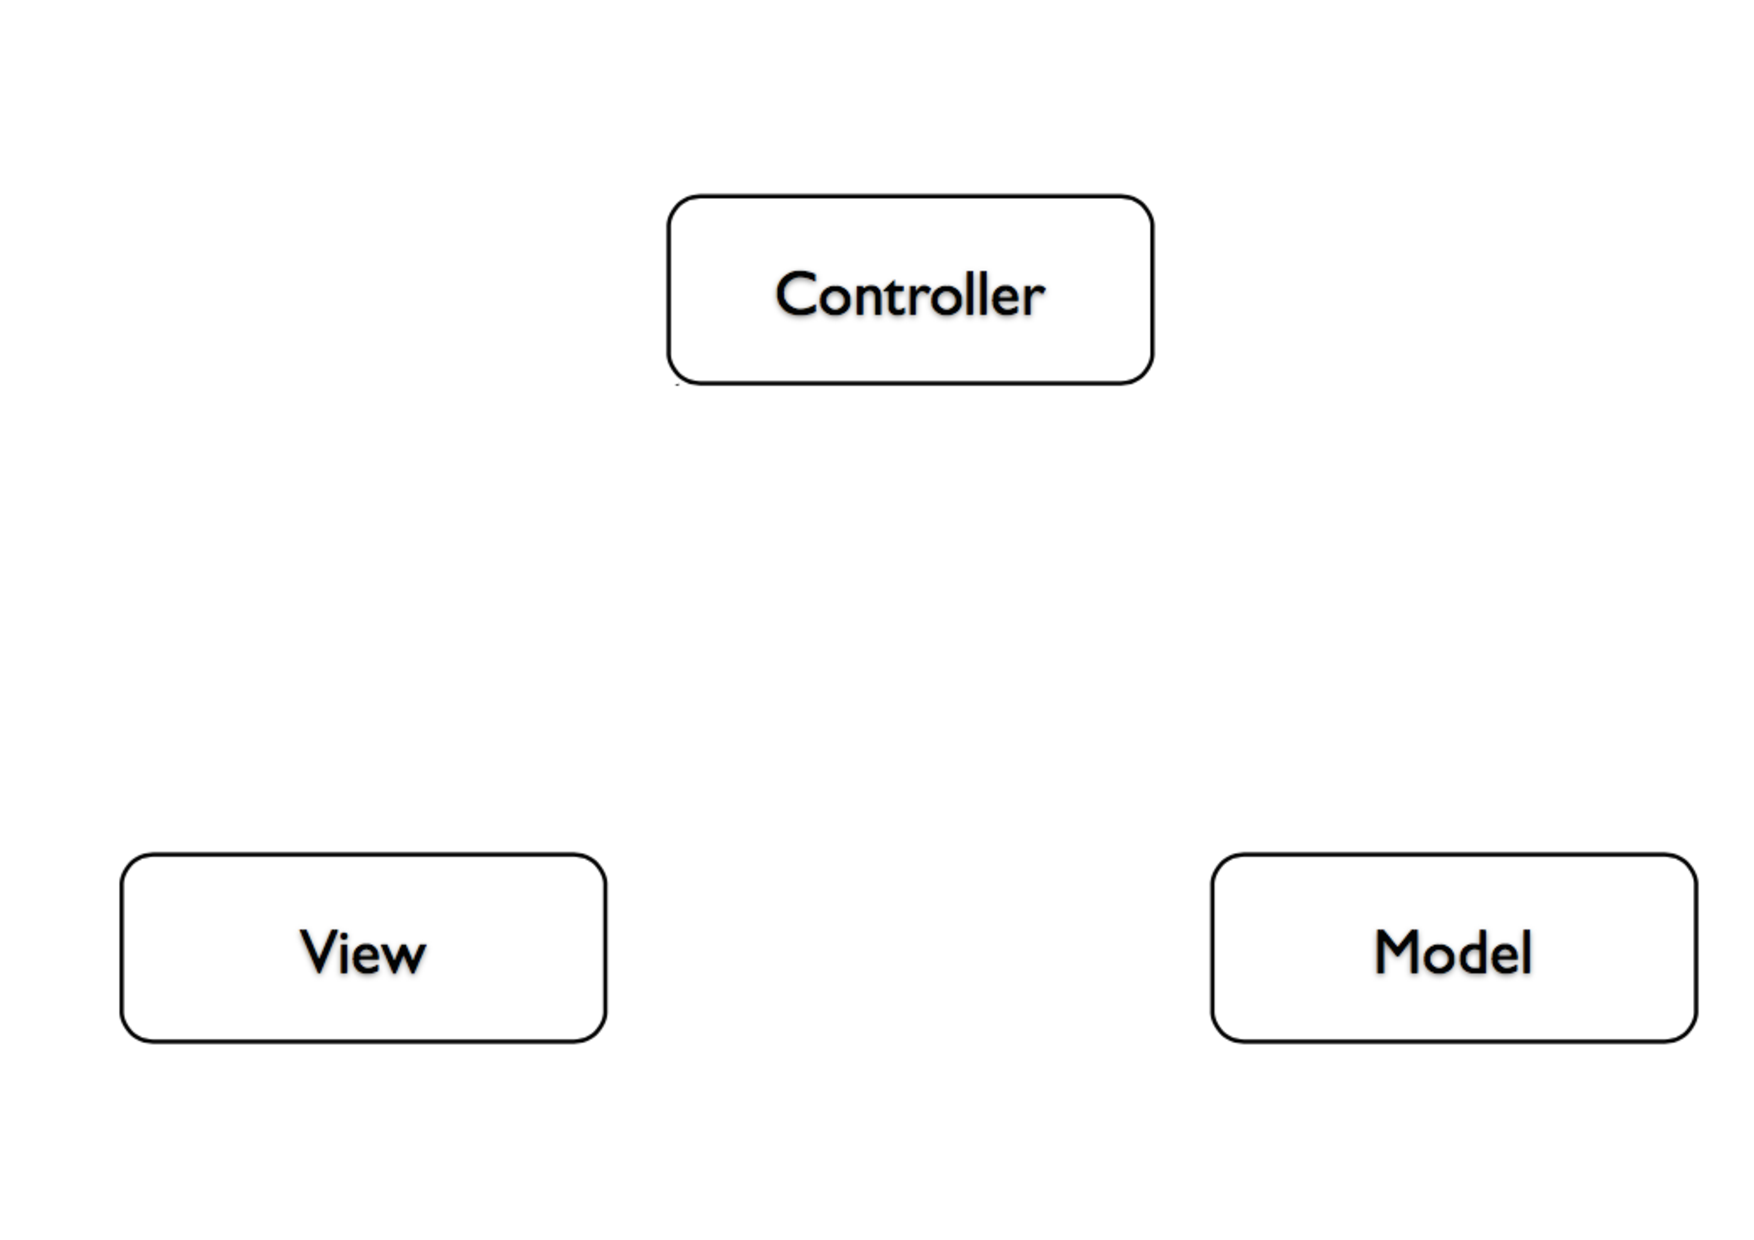
\includegraphics[width=0.5\textwidth]{Img/MVC1.pdf}
\end{figure}


\begin{itemize}
\item \emph{Model}: \`e una rappresentazione astratta del sistema che si desidera modellare. 
\begin{itemize}
\item Il modello include i dati assieme ai metodi (logica) necessari per processare questi dati. 
\item Il modello non include nessuna informazione di \emph{come} i dati sono visualizzati
\end{itemize}
\item \emph{View} (Interface): \`e solitamente attaccata ad un modello. In genere, ad un determinato modello possono essere attaccate una o pi\`u Views, ogni view \`e capace di mostrare una o pi\`u rappresentazione del modello (esempio una rappresentazione su schermo o cartacea). La view consente di:
\begin{itemize}
\item mostrare dei dati a un utente
\item essere aggiornata quando il modello cambia
\end{itemize}
\item \emph{Controller} (Coordinator): riceve gli input dalla view e li trasforma in azioni che il modello pu\`o eseguire. Delle azioni potrebbero essere il click su un bottone nel caso di una GUI o delle richieste GET e POST in una applicazione web. Il controller in alcuni casi potrebbe selezionare nuove view, per esempio nel caso delle richieste HTTP.
\end{itemize}



Interazione View-Model. Possono esserci due tipi di interazioni tra view e model:
\begin{itemize}
\item \emph{push model} la view si registra al modello e aspetta notifiche
\item \emph{pull model} la view \`e responsabile di eseguire delle query sul modello quando deve aggiornare la sua visualizzazione
\end{itemize}

\subsection{Interazione ``classica" tra i componenti dell'MVC}
Una delle possibili interazioni del Model View Controller (quella proposta inizialmente nel 1979) \`e la seguente:
 La \emph{view} osserva (pattern observer o listener) il modello. Ogni cambiamento del modello viene propagato come una notifica che la view riceve. Nota il modello non \`e direttamente consapevole di chi osserva, semplicemente manda un messaggio agli ascoltatori.
Il \emph{controller} \`e azionato dalla\begin{figure}[h]
\centering
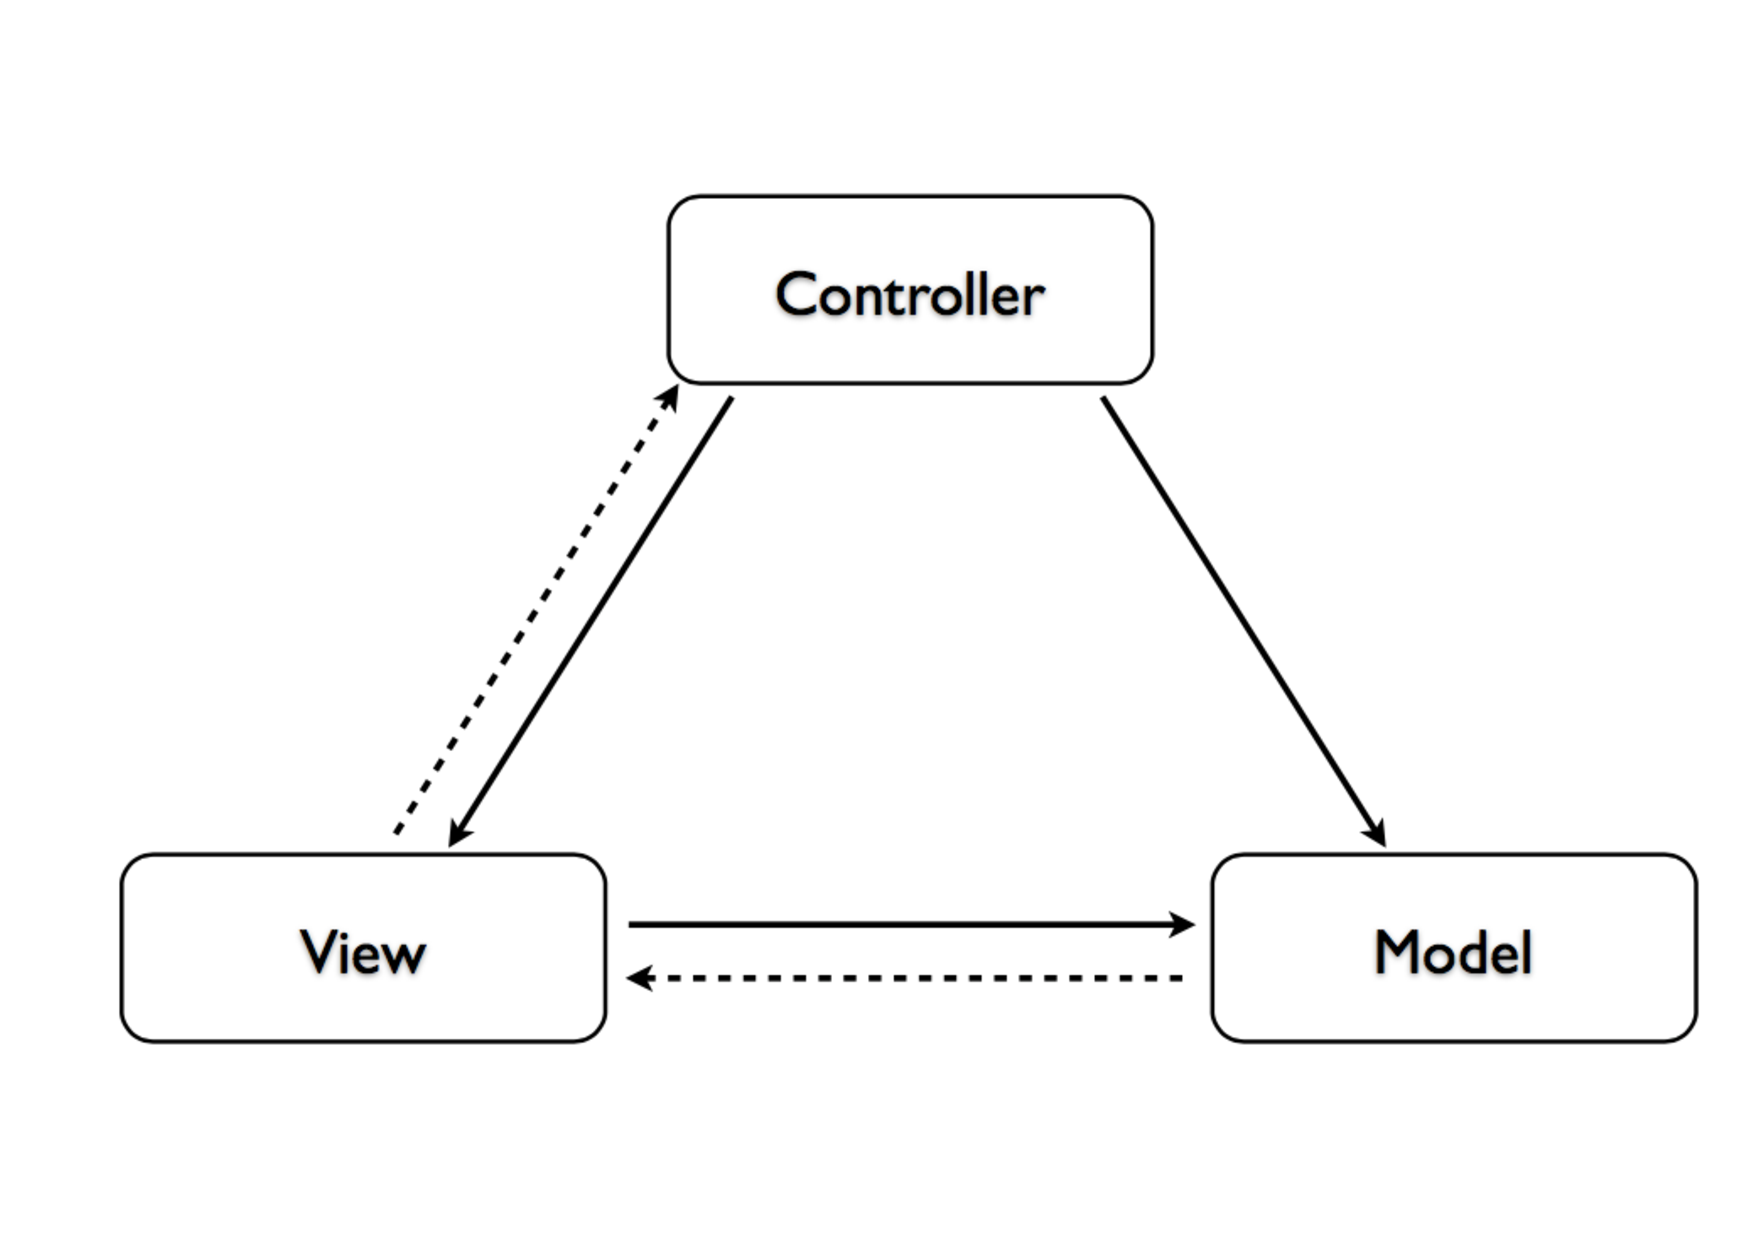
\includegraphics[width=0.5\textwidth]{Img/MVC2.pdf}
\end{figure} view (o da una sua logica interna). Quando un azione viene eseguita sulla view, una notifica viene mandata al controller. Il controller osserva la view (mediante un osservatore o un listener). Il controller conosce il modello sottostante. Quando un azione viene eseguita sulla view (un comando chiamato sull'interfaccia del server), l'azione viene segnalata al controller, il controller accede al modello e lo aggiorna in relazione all'azione dell'utente. \emph{In alcune architetture il controllore potrebbe anche essere responsabile di cambiare la view, per esempio nelle architetture enterprise di java.}




\subsection{Modifiche all'MVC}
\label{ModificheMVC}
Una modifica al pattern MVC utilizzata nei sistemi Apple consiste nel posizionare il controller tra la view e il modello. La differenza principale tra questo framework e la versione classica \`e che le notifica del cambiamento dello stato del modello sono comunicate alla view \emph{attraverso} il controller. Il controller fa da ``mediatore" tra i dati del modello e la view in entrambe le direzioni: le azioni sulla view devono passare per il controller per essere tramutate in azioni del modello. I cambiamenti del modello sono comunicati alla view dopo che sono passati per il controllore. 
In questo caso, la view chiama un metodo sul controllore, il controllore esegue l'azione sul modello, se l'azione ha provocato dei cambiamenti il modello notifica i suoi ascolatori: i controller, i quali a loro volta notificano la modifica alla view. Il controllore pu\`o essere suddiviso in altri sottocontrollori.

\begin{figure}[h]
\centering
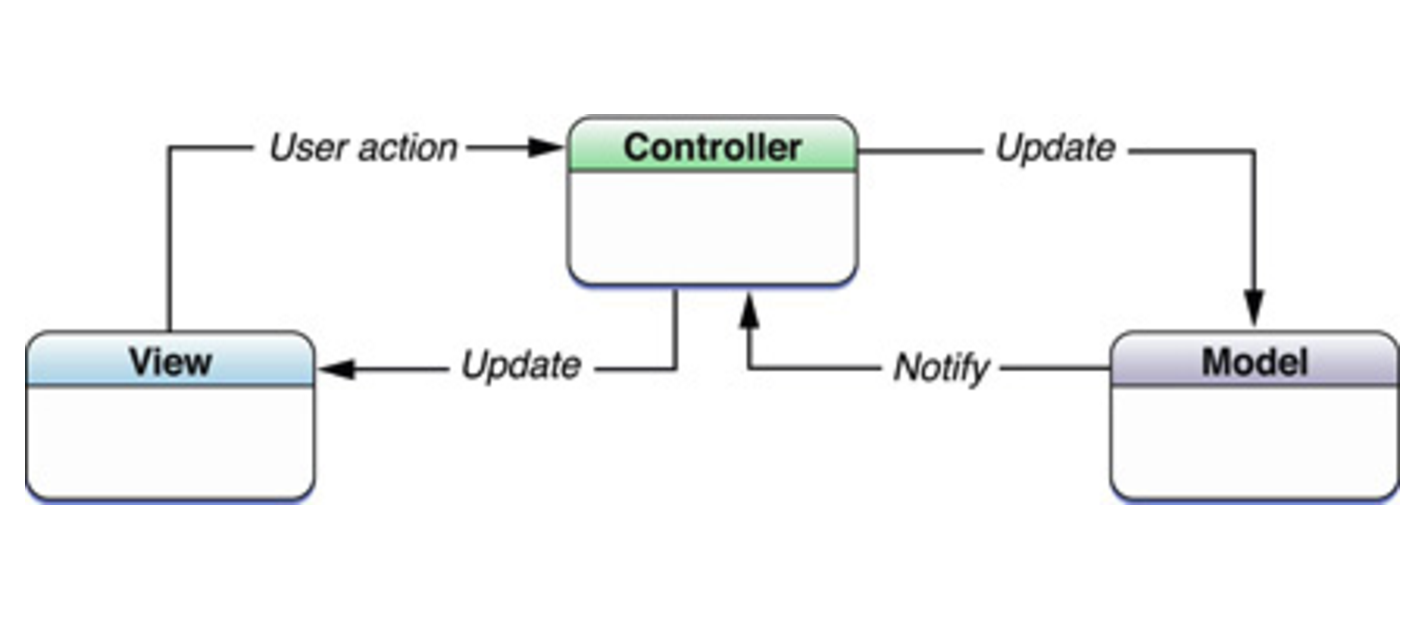
\includegraphics[width=0.7\textwidth]{Img/MVCCocoa.pdf}
\end{figure}

Per maggiori informazioni potete fare riferimento a \url{https://developer.apple.com/library/mac/documentation/General/Conceptual/DevPedia-CocoaCore/MVC.html}.

\subsection{MVC client/Server}
In un architettura client/server l'MVC pu\`o essere visto a diversi livelli di astrazione a seconda della granularit\`a con cui si affronta il problema. Se si considera ``l'applicazione finale" la view rappresenta l'interfaccia con cui il client (utenti) interagisce. In questo contesto esistono due approcci:
\begin{itemize}
\item \emph{server-side} MVC: \`e il caso in cui model, view e controller sono eseguiti sul sever. \`E per esempio il caso delle pagine HTML (View)
che vengono generate sul server
\item \emph{client-side} MVC: \`e il caso in cui model e controller sono posti sul client. \`E il caso per esempio delle applicazioni per tablet.
\end{itemize}

Se invece consideriamo come ``granularit\`a" il server, i nostri client (utenti) sono le persone che useranno le API, ovvero le interfacce della nostra applicazione (View) che esponiamo, il controllore \`e il coordinatore che gestisce l'interazione tra le view e il modello che contiene lo stato del gioco. 





%\section{Testing}
%\subsection{Test di unit\`a}
%Consentono di testare una singola entit\`a (classe o metodo). 
%\subsection{JUnit}
%JUnit \`e un framework per il test di unit\`a per il linguaggio Java e consente di seguire un paradigma di programmazione test-driven.
%
%\subsection{Unit test case}
%\begin{itemize}
%\item porzione di codice che assicura che un altra parte di codice (in genere un metodo) funziona come aspettato.
%\item un test formale ben scritto \`e caratterizzato da un input noto e un output atteso che \`e stabilito prima dell'esecuzione del test.
%\item in genere per ogni requisito (funzionalit\`a implementate) devono esserci \textbf{almeno} due test. Uno positivo e l'altro negativo
%\item junit consente di utilizzare le annotazioni per identificare i metodi di test.
%\item le asserzioni servono a confrontare i risultati ottenuti con quelli attesi
%\end{itemize}
%
%\subsection{Caratteristiche di JUnit}
%JUnit fornisce le seguenti features:
%\begin{itemize}
%\item \emph{Fixture}: \`e possibile settare uno stato predefinito degli oggetti prima di eseguire un test. L'obbiettivo \`e di assicurare che l'ambiente nel quale i test sono eseguiti \`e noto e fissato in modo che i test siano ripetibili (@Before (setting), @After (pulizia)). 
%\item \emph{Test runner}: \`e utilizzato per eseguire i test (trasparente all'utente)
%\end{itemize}
%
%\subsection{Best Practices}
%\begin{itemize}
%\item non utilizzare il costruttore del test case per settare il test case.
%\item non assumere di conoscere l'ordine nel quale i test case vengono eseguiti (anche all'interno del singolo junit).
%\item non scrivere test cases che hanno side effects 
%\item scrivere i test che leggono dati da locazioni del file sistem utilizzando path relativi
%\item memorizzare i dati che sono necessari per i test assieme ai test stessi
%\item assicurati che i nomi dei test sono time-indipendent
%\item scegliere i nomi dei  test nel modo corretto
%\begin{itemize}
%\item il nome del test deve iniziare con la parola Test (esempio \emph{TestClassUnderTest})
%\item il nome dei metodi nel test case devono descrivere cosa viene testato (esempio \emph{testLoggingEmptyMessage()})
%\end{itemize}
%\item utilizza i metodi assert e fail di junit nel modo corretto per mantenere il codice pulito. Considera per esempio la leggibilit\' a di assertEquals ("The number of credentials should be 3", 3, creds); rispetto a assert (creds == 3); 
%\item commentare i test con la javadoc
%\item mantieni i test piccoli e veloci
%\end{itemize}
%
%\subsection{Testing private methods}
%Per testare dei metodi privati ci sono 2 strade possibili:
%\begin{itemize}
%\item testarlo attraverso un altro metodo pubblico che lo utilizza
%%\item utilizzare la \emph{reflection} (nel caso sia proprio necessario).
%\end{itemize}
%%in pratica conviene testare solo la parte di codice visibile da un ipotetico “client” completamente esterno al codice, e quindi trascurare i metodi protetti
%
%\subsection{Che cosa testare?}
%Non \`e una regola assoluta, ma il principio generale \`e: \emph{quanto pi\`u una parte di codice \`e visibile dall'esterno, tanto pi\`u deve essere testata}


\section{Esercizi}



\subsection{Esercizio 1: MVC}
\begin{framed}
Gestire il seguente gioco:
Dei carcerati sono in una prigione. I poliziotti della prigione decidono di salvare i carcerati se dimostrano una capacit\`a collaborativa e una certa attitudine nel risolvere problemi. I prigionieri vengono lasciati nel cortile della prigione per un determinato tempo al fine di accordarsi relativamente a una strategia per salvarsi. Dal giorno seguente in poi un prigioniero alla volta verr\`a fatto entrare in una cella $t$ contenente un interruttore.
Un prigioniero pu\`o  entrare pi\`u volte nella cella prima che un altro prigioniero entri e ad intervalli di tempo non prefissati. L'interruttore pu\`o essere in due stati ON e OFF. Ogni prigionierio pu\`o muovere l'interruttore da ON a OFF e viceversa o lasciarlo nello stato  attuale. Tra un prigioniero e l'altro l'interruttore non viene toccato dai poliziotti. L'unica informazione che si conosce \`e che l'interruttore \`e inizialmente a OFF. Il gioco continua finch\`e uno dei prigionieri dice: ``ogni prigioniero \`e stato nella cella prima di me \emph{almeno} una volta". Se \`e corretto tutti i prigionieri sono liberati altrimenti vengono uccisi.
\end{framed}
\clearpage
\begin{figure}[h]
\centering
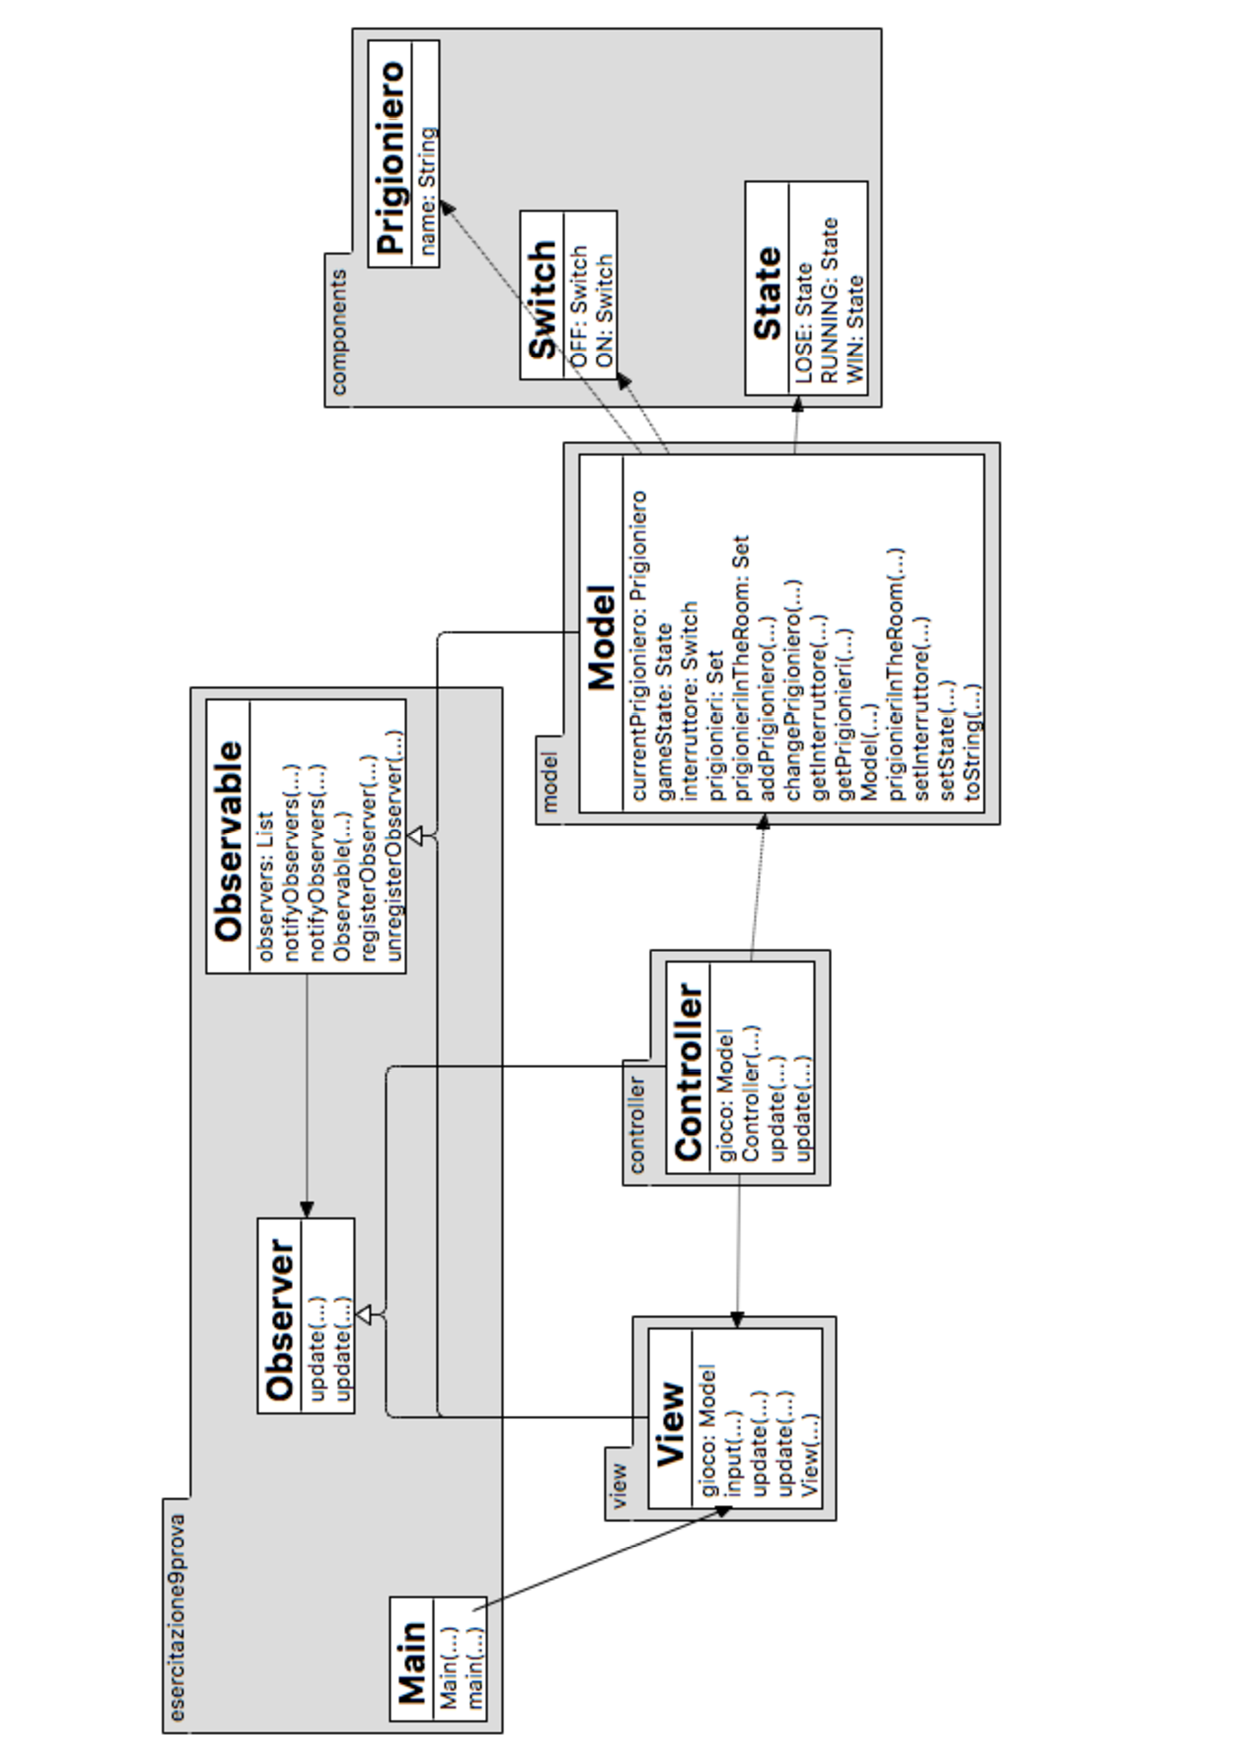
\includegraphics[width=1\textwidth]{Img/MVC.pdf}
\caption{Class diagram relativo alla soluzione dell'esercizio 1}
\label{Fig:MVCSol}
\end{figure}
\clearpage

\subsubsection{Observable/observer}
\begin{lstlisting}[language=Java]
public abstract class Observable {

	private List<Observer> observers;
	
	public Observable(){
		observers=new ArrayList<Observer>();
	}
	
	public void registerObserver(Observer o){
		observers.add(o);
	}
	
	public void unregisterObserver(Observer o){
		this.observers.remove(o);
	}
	
	public void notifyObservers(){
		for(Observer o: this.observers){
			o.update();
		}
	}
	public <C> void notifyObservers(C c){
		for(Observer o: this.observers){
			o.update(c);
		}
		
	}	
}

\end{lstlisting}


\begin{lstlisting}[language=Java]
public interface Observer {

	public void update();
	public <C> void update(C change);
}
\end{lstlisting}


\subsubsection{Model}

\begin{lstlisting}[language=Java]
public enum State {
	RUNNING, WIN, LOSE
}
\end{lstlisting}

\begin{lstlisting}[language=Java]
public enum Switch {
	ON, OFF
}
\end{lstlisting}

\begin{lstlisting}[language=Java]
public class Prigioniero {

	private final String name;
	
	public Prigioniero(String name){
		this.name=name;
	}

	@Override
	public String toString() {
		return "Prigioniero [name=" + name + "]";
	}

	public String getName() {
		return name;
	}
	
	@Override
	public int hashCode() {
		final int prime = 31;
		int result = 1;
		result = prime * result + ((name == null) ? 0 : name.hashCode());
		return result;
	}

	@Override
	public boolean equals(Object obj) {
		if (this == obj)
			return true;
		if (obj == null)
			return false;
		if (getClass() != obj.getClass())
			return false;
		Prigioniero other = (Prigioniero) obj;
		if (name == null) {
			if (other.name != null)
				return false;
		} else if (!name.equals(other.name))
			return false;
		return true;
	}
}
\end{lstlisting}

\begin{lstlisting}[language=Java]
public class Model extends Observable{

	private Set<Prigioniero> prigionieri;
	private Set<Prigioniero> prigionieriInTheRoom;
	private Prigioniero currentPrigioniero;
	private Switch interruttore;
	private State gameState;
	
	public Model() {
		prigionieri=new HashSet<Prigioniero>();
		prigionieriInTheRoom=new HashSet<Prigioniero>();
		this.addPrigioniero(new Prigioniero("Luca"));
		this.addPrigioniero(new Prigioniero("Pietro"));
		this.addPrigioniero(new Prigioniero("Paolo"));
		this.interruttore=Switch.OFF;
		gameState=State.RUNNING;
		this.changePrigioniero();
	}
	
	public void setState(State state){
		this.gameState=state;
		System.out.println("I am the model I am notifying my observers with a new game state");
		
		this.notifyObservers(gameState);
	}
	
	public void addPrigioniero(Prigioniero prigioniero){
		currentPrigioniero=prigioniero;
		this.prigionieri.add(prigioniero);
	}

	public Switch getInterruttore() {
		return interruttore;
	}
	
	public Set<Prigioniero> getPrigionieri(){
		return Collections.unmodifiableSet(this.prigionieri);
	}
	public Set<Prigioniero> prigionieriInTheRoom(){
		return Collections.unmodifiableSet(this.prigionieriInTheRoom);
	}
	
	
	public void setInterruttore(Switch value){
		this.interruttore=value;

	}
	
	public void changePrigioniero(){
		List<Prigioniero> prigionieriList=new ArrayList<Prigioniero>(prigionieri);
		Collections.shuffle(prigionieriList);
		this.currentPrigioniero=prigionieriList.get(0);
		this.prigionieriInTheRoom.add(currentPrigioniero);
		System.out.println("I am the model I am notifying my observers");
		
		this.notifyObservers();
	}
	
	@Override
	public String toString() {
		return "Gioco [currentPrigioniero=" + currentPrigioniero
				+ ", interruttore=" + interruttore + "]";
	}
}
\end{lstlisting}

\subsubsection{Azioni}

\begin{lstlisting}[language=Java]
public abstract class Action {

	private final Model gioco;
	
	public Action(Model gioco){
		this.gioco=gioco;
	}
	
	protected Model getGioco(){
		return this.gioco;
	}
	
	public abstract void esegui();
}
\end{lstlisting}

\begin{lstlisting}[language=Java]
public class Scommetti extends Action{

	public Scommetti(Model gioco) {
		super(gioco);
	}

	@Override
	public void esegui() {
		if(this.getGioco().prigionieriInTheRoom().containsAll(this.getGioco().getPrigionieri())){
			this.getGioco().setState(State.WIN);
		}
		else{
			this.getGioco().setState(State.LOSE);
		}
		
	}
}
\end{lstlisting}

\begin{lstlisting}[language=Java]
public class TurnOff extends Action{

	public TurnOff(Model gioco) {
		super(gioco);
	}

	@Override
	public void esegui() {
		this.getGioco().setInterruttore(Switch.OFF);
		this.getGioco().changePrigioniero();
	}
}
\end{lstlisting}

\begin{lstlisting}[language=Java]
public class TurnOn extends Action{

	public TurnOn(Model gioco) {
		super(gioco);
	}

	@Override
	public void esegui() {
		this.getGioco().setInterruttore(Switch.ON);
		this.getGioco().changePrigioniero();
	}
}
\end{lstlisting}

\subsubsection{Controller}
\begin{lstlisting}[language=Java]
public class Controller implements Observer {

	private final Model gioco;

	public Controller(Model gioco, View view) {
		this.gioco = gioco;
		view.registerObserver(this);
	}

	public <C> void update(C change) {
		System.out.println("I am the controller I have been notified by the view with an action C");
		Action azione;
		if (change.equals(Switch.ON.toString())) {
			azione = new TurnOn(this.gioco);
		} else {
			if (change.equals(Switch.OFF.toString())) {
				azione = new TurnOff(gioco);
			} else {
				
				azione = new Scommetti(gioco);
			}
		}
		azione.esegui();
	}

	public void update() {
		System.out.println("I am the controller I have been notified by the view");

	}
}
\end{lstlisting}

\subsubsection{View}
\begin{lstlisting}[language=Java]
public class View extends Observable implements Observer {

    //ATTENZIONE!
    // IN GENERALE NON E' UNA BUONA PRATICA FORNIRE ALLA VIEW UN 
    //REFERENCE AL MODELLO 
    // INFATTI, CON QUESTA SCELTA SAREBBE POSSIBILE MODIFICARE
    // IL MODELLO SENZA PASSARE PER IL CONTROLLER
	private final Model gioco;
	
	public View(Model gioco) {
		gioco.registerObserver(this);
		System.out.println(gioco);
		this.gioco=gioco;
	}

	public void input(String input) {
		System.out.println("I am the view I am notifying my observers");
		this.notifyObservers(input);
	}

	public void update() {
		System.out.println("I am the view I have been notified by the model ");
		System.out.println(gioco);
	}

	public <C> void update(C change) {
		System.out.println("I am the view I have been notified by the model with an update C");
		
		if (change.equals(State.WIN)) {
			System.out.println("Avete vinto");
		} else {
			System.out.println("Siete morti");
		}
		System.exit(0);

	}

}
\end{lstlisting}

\subsubsection{Main}
\begin{lstlisting}[language=Java]
public class Main {

	public static void main(String[] args) throws IOException {
		Scanner in = new Scanner(System.in);
		Model gioco=new Model();
		View view =new View(gioco);
		Controller controller=new Controller(gioco, view);
		
		while(true){
			System.out.println("Dimmi il comando ON/OFF ");
			String comando = in.nextLine();
			view.input(comando);
		}
	}
}
\end{lstlisting}

\subsection{Esercizi per casa}
Provare a implementare la versione ``modificata" dell'MVC presentata in~\ref{ModificheMVC}.


%\subsection{Esercizio 2: Testing}
%\begin{framed}
%Vogliamo creare un metodo che converte dollari in franchi svizzeri (CHF).
%\end{framed}
%
%\textbf{Requisito base}.
%Dobbiamo essere capaci di moltiplicare un numero per un altro. 
%Esempio se il cambio Dollari-CHF 2 :1, 5 Dollari vengono convertiti in 10 franchi.
%
%\begin{itemize}
%\item Visto che siamo test driven partiamo dai test e non dagli oggetti
%\item File $>$ new $>$ Junit Test Case (Test)
%\item scegliamo il nome del test TestMultiplication. Nota il nome del test deve iniziare con la parola \textbf{Test} e deve essere chiara la funzionalit\`a testata
%\end{itemize}
%\subsubsection{Step 1}
%\textbf{Step 1.1 Creating the test}
%
%\begin{lstlisting}
%package org.ingsoft.junit;
%
%import static org.junit.Assert.*;
%
%import org.ingsoft.junit.tdd.Dollar;
%import org.junit.Test;
%
%public class TestMultiplication {
%	@Test
%	public void test() {
%		Dollar five=new Dollar(5);
%		five.times(2);
%		assertEquals(10, five.amount);
%	}
%}
%\end{lstlisting}
%
%Problemi: public fields, side effects, integer for monetary amounts.
%
%Vogliamo compilare il prima possibile. Cosa dobbiamo fare?
%\begin{itemize}
%\item Creare la classe dollaro
%\item Creare un costruttore
%\item Creare il metodo times
%\item Creare l'attributo pubblico  amount
%\end{itemize}
%
%\textbf{Step 1.2 Making the test running}
%\begin{lstlisting}
%package org.ingsoft.junit.tdd;
%public class Dollar {
%	
%	public int amount=0;
%	
%	public Dollar(int value){
%		
%	}
%	public void times(int value){
%		    
%	}
%}
%\end{lstlisting}
%Compila perfetto. Problema il test non \`e passato.
%
%\begin{lstlisting}
%package org.ingsoft.junit.tdd;
%public class Dollar {
%	
%	public int amount=10;
%	
%	public Dollar(int value){
%		
%	}
%	public void times(int value){
%	}
%}
%\end{lstlisting}
%Compila perfetto il test \`e passato.
%
%\textbf{Step 1.3 Refactor}\\
%C'\`e una dipendenza tra il codice e il test. Ovvero abbiamo del codice duplicato (il numero 10). Come possiamo eliminarlo?
%\begin{itemize}
%\item Passo  1: nel metodo  times scriviamo this.amount = 5*2 
%\item Passo 2: da dove possiamo ottenere il 5?  
%\begin{itemize}
%\item Mettiamo nel costruttore this.amount=value;
%\item Mettiamo nella metodo times  this.amount = this.amount*2 
%\end{itemize}
%\item Passo 3: da dove possiamo ottenere il 2?
%\begin{itemize}
%\item mettiamo nel metodo times  this.amount = this.amount* value
%\end{itemize}
%\item Passo 4: rimuoviamo il codice replicato
%\begin{itemize}
%\item  replace amount = amount* value with amount *= value
%\end{itemize}
%\end{itemize}
%
%\subsubsection{Step 2}
%Problema dopo aver eseguito un operazione l'oggetto dollaro cambia.\\
%\textbf{Step 2.1 Creating the test}\\
%\begin{lstlisting}
%package org.ingsoft.junit;
%
%import static org.junit.Assert.*;
%
%import org.ingsoft.junit.tdd.Dollar;
%import org.junit.Test;
%
%public class TestMultiplication {
%	@Test
%	public void test() {
%		Dollar five=new Dollar(5);
%		five.times(2);
%		assertEquals(10, five.amount);
%		five.times(3);
%		assertEquals(15, five.amount);
%	}
%}
%\end{lstlisting}
%
%
%\textbf{Step 2.2 Making the test running}\\
%Cambiare l'interfaccia della classe dollaro per fagli ritornare un nuovo oggetto.
%\begin{lstlisting}
%@Test
%	public void test() {
%		Dollar five=new Dollar(5);
%		Dollar product=five.times(2);
%		assertEquals(10, product.amount);
%		product=five.times(3);
%		assertEquals(15, product.amount);
%	}
%\end{lstlisting}
%
%\begin{lstlisting}
%package org.ingsoft.junit.tdd;
%
%public class Dollar {
%	
%	public int amount;
%	
%	public Dollar(int value){
%		this.amount=value;
%	}
%	public Dollar times(int value){
%		this.amount *= value;
%		return null;
%	}
%}
%\end{lstlisting}
%
%
%\begin{lstlisting}
%public Dollar times(int value){
%		return new Dollar(this.amount *= value);
%	}
%\end{lstlisting}
%
%
%
%\textbf{Step 2.3 Refactor}\\
%Posso mettere l'attributo amount come privato.
%
%\subsection{Esercizio 3: Testing}
%\begin{framed}
%Vogliamo creare un account bancario
%\end{framed}
%Test 1: all'inizio il saldo deve essere 0
%\begin{lstlisting}
%public class BankAccountTest {
%
%	/**
%	 * devo testare un BankAccount quindi creo il
%	 * campo nella classe di test
%	 */
%	private BankAccount account=null;
%	@Test
%	public void test() {
%		fail("Not yet implemented");
%	}
%}
%\end{lstlisting}
%Non compila, implementiamo il minimo possibile per far compilare il test
%\begin{lstlisting}
%\end{lstlisting}
%
%Il test fallisce, vediamo di porre rimedio.
\clearpage

% ---- Bibliography ----




%\addcontentsline{toc}{chapter}{Bibliography}
%\bibliographystyle{alpha}
%\bibliography{bib}
\nocite{*}


\end{document}

